%%%%%%%%%%%%%%%%%%%%%%%%%%%%%%%%%%%%%%%%%
% University/School Laboratory Report
% LaTeX Template
% Version 3.1 (25/3/14)
%
% This template has been downloaded from:
% http://www.LaTeXTemplates.com
%
% Original author:
% Linux and Unix Users Group at Virginia Tech Wiki 
% (https://vtluug.org/wiki/Example_LaTeX_chem_lab_report)
%
% License:
% CC BY-NC-SA 3.0 (http://creativecommons.org/licenses/by-nc-sa/3.0/)
%
%%%%%%%%%%%%%%%%%%%%%%%%%%%%%%%%%%%%%%%%%

%----------------------------------------------------------------------------------------
%	PACKAGES AND DOCUMENT CONFIGURATIONS
%----------------------------------------------------------------------------------------

\documentclass{article}

\usepackage{graphicx} % Required for the inclusion of images
\usepackage{natbib} % Required to change bibliography style to APA
\usepackage{amsmath} % Required for some math elements 
\usepackage{amsthm}
\usepackage[hyphens]{url}
\usepackage{hyperref}
\usepackage{subcaption}
\usepackage{float}
\usepackage{array}
\usepackage{amssymb}


\setlength\parindent{0pt} % Removes all indentation from paragraphs

\newtheorem*{remark}{Theorem}
\newtheorem*{definition}{Definition}

%\renewcommand{\labelenumi}{\alph{enumi}.} % Make numbering in the enumerate environment by letter rather than number (e.g. section 6)

%\usepackage{times} % Uncomment to use the Times New Roman font

%----------------------------------------------------------------------------------------
%	DOCUMENT INFORMATION
%----------------------------------------------------------------------------------------

\title{Homework \#3 \\RSA \\[0.2em]\small{}CNS Course Sapienza} % Title and subtitle

\author{Riccardo \textsc{Prinzivalle}, 1904064} % Author name

\date{November 20, 2020} % Date for the report

\begin{document}

\maketitle % Insert the title, author and date

%----------------------------------------------------------------------------------------
%	SECTION 0
%----------------------------------------------------------------------------------------

\section{Homework Goal}

This homework contains an implementation of RSA algorithm based on major libraries for the mathematical functions, a comparison with the insecure \textit{PyCryptoDome} RSA and with the \textit{PyCryptoDome} AES.

%----------------------------------------------------------------------------------------
%	SECTION 1
%----------------------------------------------------------------------------------------

\section{RSA Implementation}

RSA basically is divided in two part: the initialization and the encryption.\newline 
The encryption phase is simpler than the initialization: it uses only an exponentiation and a modulo reduction. The modulo reduction is already implemented in python (used in this homework), instead what it is needed is an efficient implementation of the exponentiation. To do so, I used the proposed \textbf{Square And Multiply} in the slides of the course: at first with small values of base and exponent it worked flawlessly, but during the test with bigger messages and keys, the computation explodes, so I thought to reduce in modulo after every performed computation (since we have to do it after the exponentiation, so why don't do it at every step?) and the \textbf{SAM} computation time dropped to some seconds. The code can be seen in Fig. \ref{fig:sam}

\begin{figure}[H]
	\centering
	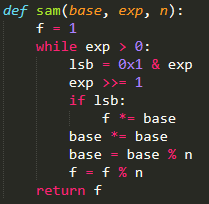
\includegraphics[width=0.345\linewidth]{images/SAM.png}
	\caption{Improved version of Square And Multiply}
	\label{fig:sam}
\end{figure}

Now the easy task is done; the initialization is the part which requires more attention to guarantee the security of our implementation. The operation to be performed are:

\begin{enumerate}
	\item find two large prime numbers $p$ and $q$
	\item compute $n = p \cdot q$
	\item compute Euler Phi function as $\Phi(n) = (p-1)(q-1)$ exploiting prime properties of $p$ and $q$
	\item select an exponent $e \in {1, 2, \dots, \Phi(n)}$ such that $gcd(e, \Phi(n) = 1$
	\item compute $d$ such that $d \cdot e = 1 \mod \Phi(n)$
\end{enumerate}

Now every operation will be analyzed in more depth.\newline
The first step is quite complicate: the machine, a deterministic entity, must find randomically two numbers in an unpredictable way, we have to use them in cryptography so no one must be able to exploit some not true random generations. As explained in \cite{primeNum}, the idea is to let the computer generate a random number of the dimension we need and then test if it is a prime or not; that is possible since the dimension of the number we need for RSA encryption still guarantees to obtain a good enough probability to obtain a prime, this probability decreases as the order of the generated number increases. The problem is how to generate these random numbers: as stated in \cite{TRNG}, we cannot simply use a pseudo random number generator, it will generate numbers that are only apparently random, and this property can be exploited by an attacker to find a pattern in these random numbers. The most secure way to generate a random number is to have a true random number generator, which uses some environment input to have a source of true randomization, the problem is that these generator are hard to design and costly o implement. This source \cite{TRNG} explains also that it is possible to find some services on the internet that claim to have TRNG, but for this implementation it will be used the idea of \cite{pyrandom}: we can use cryptography secure random number generator, which uses some special source of randomization from outside the computer to initialize a random number generator. This is done by using an utility from \textit{PyCryptoDome} that generates random numbers (in this implementation it has been specified to use os.urandom, which is cryptographically secure, but I have a doubt if it check to have enough entropy in the pool or has the same behavior specified in slide 8 about prime numbers) and then performs the primality test. \newline
The second step perform this multiplication in order to have the number $n$ composed only by two prime factors, and this property will be exploited in th next step. \newline
The third step computes the Totient function by exploiting the previous step property and using simpler computations. \newline
The fourth and the fifth step are implemented together in this work: since in the fourth step we need to compute the GCD, this can be done trough the \textbf{Extended Euclidean Algorithm} needed in the fifth step. To select the exponent it is used SystemRandom, which uses and delegates to the underlining system to compute the random number and in addition it has already implemented the possibility to add from which choosing the random number, as it is needed in the fourth step. As already said, the GCD test is performed by the EEA algorithm, which is needed to compute $d$. The EEA implementation is iterative, it is based on the slide pseudocode with some improvements, on the net I was able to find also a recursive version, maybe it has more performance, but since RSA needs big numbers, the recursive version reached the limit number of recursive executions.

%----------------------------------------------------------------------------------------
%	SECTION 3
%----------------------------------------------------------------------------------------

\section{RSA Comparison}

\renewcommand{\arraystretch}{2}

\begin{table}[H]
	\begin{center}
		\begin{tabular}{ |c || c | c | c | c | c | c | }
			\hline
			Algorithm Family & Cryptosystems & \multicolumn{4}{c |}{Security Level (bit)}\\
			& & 80 & 128 & 192 & 256\\ [0.5ex] 
			\hline\hline
			Integer Factorization & RSA & 1024 & 3072 & 7680 & 15360  \\ 
			
			Discrete Logarithm & DH, DSA, Elgamal & 1024 & 3072 & 7680 & 15360  \\ 
			
			Elliptic Curves & ECDH, ECDSA & 160 & 256 & 384 & 512  \\ 
			\hline
			Symmetric key & AES, 3DES &  80 & 128 & 192 & 256  \\ 
			\hline
		\end{tabular}
		\caption{Key length comparison in public key and symmetric key algorithm}
		\label{tab:keyLen}
	\end{center}
\end{table}

%----------------------------------------------------------------------------------------
%	SECTION 4
%----------------------------------------------------------------------------------------

\section{Conclusion}

After this brief introduction on elliptic curves, it is obvious why they have been widely adopted in many cases of asymmetric encryption: they use less bits for the same level of security, so are more efficient to compute and their base concepts are easier to visualize. As suggested on section \ref{sec:use}, EC can be easily used in hybrid encryption scheme, in the key exchange phase.

%----------------------------------------------------------------------------------------
%	BIBLIOGRAPHY
%----------------------------------------------------------------------------------------

\bibliographystyle{abbrv}

\bibliography{biblio}

%----------------------------------------------------------------------------------------


\end{document}